\chapter{Conclusions and Future work}
This chapter summarizes key findings and conclusions drawn from this project,
and it will also outline potential future work and improvements that can be made.

In this paper, we have explored the use of IoT technologies in an agricultural setting. I presented 
the advantages of using IoT for monitoring and managing  agricultural processes. A prototype as also
presented, which demonstrated the proof of concept for use of IoT in agriculture. 
We also explored the use of LoRa technologies for long-range communication. 

\section{Future Work and Improvements}
At the completion of this project, I found that there are several areas for future work and improvements.
I will outline them in the following order: I will start with the sensors, then I will move on
to the firmware, backend, and finally the frontend. The first area of improvement represents the sensors used.
If I were to redo this project, I would use more qualitative sensors, because 
the sensors used in this project were not very reliable. For example the water temperature sensor
was not working properly. I would also have used more agricultural specialized sensors,
to get multiple readings from the soil and air, but that can be done in the future.

The second area of improvement is the firmware.
The firmware is not very well optimized, the code is not the cleanest and it can be improved.
I would also like to use a single sensor per node, and to have separate nodes for actuators.
This would also help reduce the complexity of the firmware and of the script that runs on the gateway.
The hardware setup can also be improved, by using a lora adapter for the Raspberry Pi,
instead of using another microcontroller. This would have also reduced the complexity of the system.
On the hardware side, a better gateway register system can be implemented. To avoid duplication 
of messages a RSSI based system can be implemented, which would allow the node to connect
to the gateway with the best signal strength. See \cite{lora_gateway_rssi} for more details.

\begin{figure}[ht]
    \centering
    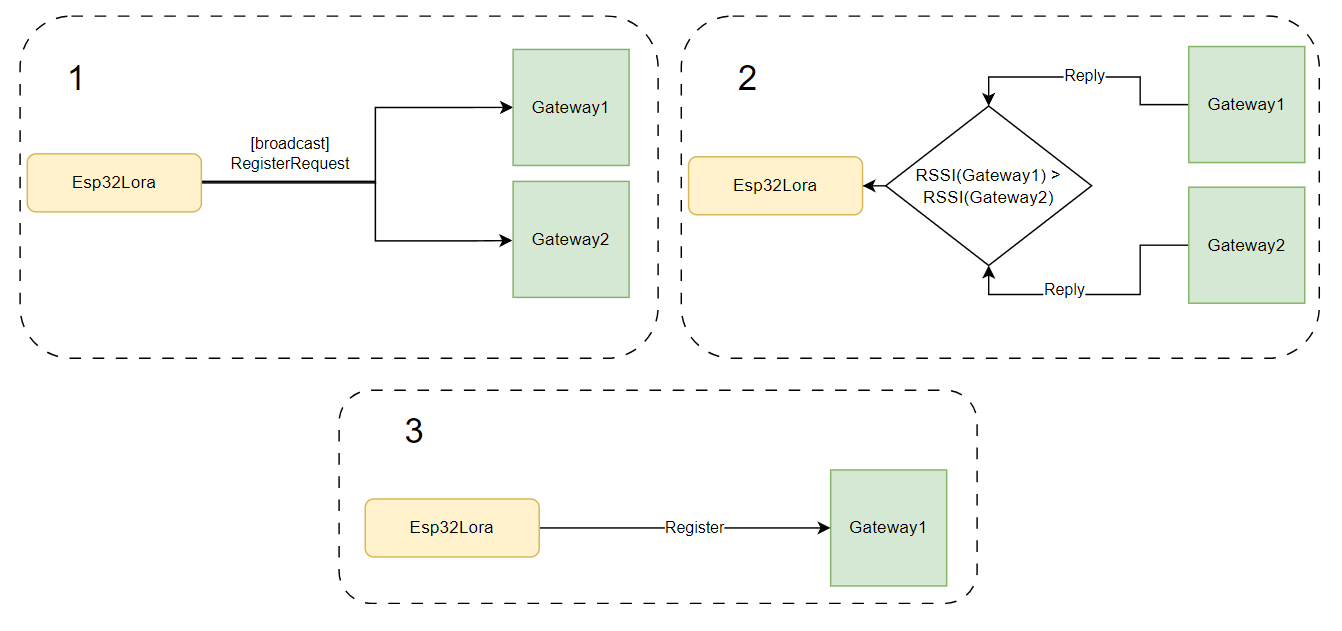
\includegraphics[width=0.6\textwidth]{images/RSSI-mechanism.png}
    \caption{RSSI based gateway registration mechanism.}
    \label{fig:lora_gateway_rssi}
\end{figure}

The third area of improvement is the backend. In the current implementation, the backend in only
one service that handles all. In the future, I would split the backend into multiple services,
each handling a specific set of tasks, such as data storage, user management, irrigation management
notifications, etc. This would allow for better scalability and maintainability of the system. It would
also allow for better security and better robustness. Beside this improvement, I would also like
to use a separate database for the sensor readings, more specifically, a time-series database.

The last area of improvement is the frontend. In my opinion, the UI design looks good, but the code 
is not the cleanest, I would like to create a even more modular design, with better separation of responsabilities.
A feature that I would like to add is the ability to see each node's position on a map,
and to be able to see the readings from each node on the map. This will allow the users
to better visualize the data and better understand the reading from each node. 
Another feature would be using of machine learning. It would be interesting to collect the data from the system,
and together with weather forecasts, to feed a machine learning model, 
which would be able to predict the best time to irrigate the crops.
